\cleartorightpage
\setcounter{NAT@ctr}{-1}
\chapter*{}\label{chapter:htsget}
\phantomsection\addcontentsline{toc}{section}{HTSget}

\begin{figure}[t!]
\centering

\includegraphics[height=10em]{chapters/htsget.png}
\end{figure}
\vspace{-4cm}


\articletitle{FAIR Data Retrieval for Sensitive Clinical Analysis in Galaxy}

Jasper Ouwerkerk\textsuperscript{\ref{htsget-affil:emc}§},
Helena Rasche\textsuperscript{\ref{htsget-affil:emc}§},
Dylan Spalding,
Saskia Hiltermann\textsuperscript{\ref{htsget-affil:emc}},
Andrew P. Stubbs\textsuperscript{\ref{htsget-affil:emc}}

{\color{chaptergrey}{§}} These authors contributed equally to this work.

\textbf{Published in:} \emph{GigaScience}, TODO \\
\doi{TODO}

\small
\begin{enumerate}
 \itemsep-0.5em
 \item Erasmus Medical Center, Clinical Bioinformatics Group, Department of Pathology, Wytemaweg 8, 3015 CN, Rotterdam, The Netherlands.\label{htsget-affil:emc}
\end{enumerate}
\normalsize


\section*{Abstract}
\textbf{Background},
In clinical research data has to be accessible and reproducible, but analyses are becoming larger and more complex. Here we propose a platform for FAIR data access and creating reproducible findings. Standardised access to a major genomic repository, the European Genome-Phenome Archive (EGA), has been achieved with API services like PyEGA3. We aim to provide a FAIR data analysis service in Galaxy by retrieving genomic data from the EGA and provide a generalised ``omics'' platform for FAIR data analysis.

\textbf{Results},
To demonstrate this, we implemented an end-to-end Galaxy workflow to replicate the findings from an RD-Connect synthetic dataset Beyond the 1 Million Genomes (synB1MG) available from the EGA. We developed the PyEGA3 connector within Galaxy to easily download multiple datasets from the EGA. We added the clin.iobio tool, a diagnostic environment for precision genomics, to Galaxy and demonstrate that it provides a more dynamic and interpretable view for trio analysis results. We developed a Galaxy trio analysis workflow to determine the pathogenic variants from the synB1MG trios using the GEMINI and clin.iobio tool. The complete workflow is available at WorkflowHub and an associated tutorial was created which helps researchers who are unfamiliar with Galaxy to run the workflow.

\textbf{Conclusions},
We showed the feasibility of reusing data from the EGA in Galaxy via PyEGA3 and validated the workflow by re-discovering spiked-in variants in synthetic data. Finally, we improved existing tools in Galaxy and created a workflow for trio analysis to demonstrate the value of FAIR genomics analysis in Galaxy.

\section*{Findings}
\label{sec:finding}

\subsection*{Background}
In the last few years there have been many developments in Findable, Accessible, Interoperable, and Reusable (FAIR) data \cite{Inau2021}. FAIR data is data and corresponding metadata which are 1) findable by both machines and humans, 2) accessible using a standard open protocol, 3) interoperable so it can easily be processed and analysed, 4) resuable so the data can be understood by anyone and make analyses reproducible \cite{fair}. FAIR data allows researchers to reanalyse data with new genetic analysis tools not yet available at the time of data publication. For example, in a study on fusion genes, 24 novel fusion in breast cancer were found with the introduction of a new tool \cite{FusionCatcher}. 

However, for many biomedical analyses, researchers are required to have considerable knowledge on using analysis tools. Moreover, many tools require knowledge of Unix commands or python coding. \cite{SnpEff, samtools, circos}. This creates a barrier for clinical researchers that want to reanalyse data, reducing the adoption of implementing FAIR principles and reanalyses.

The Galaxy platform \cite{galaxy} supports researchers in adopting these complex computation tools for their FAIR data analysis. Galaxy is an online analysis platform with a plethora of tools to perform text/table processing, omics analysis, machine learning, image analysis, and more. All these tools are maintained and developed by a growing community. Using the tools does not require any programming skills and are easy to share with colleagues and other researchers. At the end of the analysis the workflow of tools can be exported to reproduce the analysis \cite{galaxy}. These workflows can be made discoverable by uploading the workflow to WorkflowHub \cite{workflowhub}, a registry for describing, sharing, and publishing scientific computational workflows. In addition, Galaxy already has 300+ tutorials describing workflows on genome assembly, ecology, meta-genomics, variant analysis and more \cite{GTNstats}. This is beneficial to many researchers since there are many complex Unix-based tools which are essential for biomedical research. An example of such an application is Circos \cite{circos}, which is a complicated visualization tool for comparing whole genomes. This tool has been implemented within Galaxy, which makes it simple for any researcher to create Circos plots \cite{galactic-circos}.

Even though Galaxy is a well-established platform for analysis, it still lacks applications for retrieving access-controlled data from large repositories like the EGA. The EGA controls the accessibility to datasets using Data Access Committees (DACs). Requestors can access data from the EGA by contacting the DAC for the dataset of interest. DACs are generally formed by the organization which collected the data and performed the analysis. This allows researchers to access datasets of interest and also manage the accessibility of their data at the EGA \cite{DAC}.

In this work we implemented PyEGA3 \cite{EGA}, a tool which can access controlled data from the EGA, within Galaxy. Here access to datasets is managed via the EGA. Our implementation of the PyEGA3 tool allows to filter datasets, available on the EGA, based on their metadata and scale up analysis. This will be showcased by validating our workflow for trio analysis on family trios from the Beyond 1 Million Genomes (B1MG) project \cite{B1MG}. In trio analysis the differences in DNA between the maternal, paternal, and affected child i.e., proband, is analysed to detect causative variants causing a particular disease in the proband. To perform the trio-analysis we added  gene.iobio, a standalone web-based tool, to Galaxy \cite{geneiobio}. The complete workflow, including data retrieval with PyEGA3, is implemented within Galaxy and uploaded to WorkflowHub for discoverability. In addition, we wrote a tutorial to explain our workflow in detail, which is associated with the Galaxy Training Network (GTN) \cite{GTN}. This study shows it is feasible to adopt end-to-end scalable FAIR analysis of clinical data, and ultimately for any future analysis on data available at the EGA. 

\subsection*{Results}

\subsubsection*{PyEGA3}
PyEGA3 was implemented to retrieve access controlled data from the EGA in Galaxy. Authentication of the user is done by password and username. This information is encrypted using a Vault abstraction \cite{vault} when configured by the Galaxy administrator. In addition, LS Login (Previously ELIXIR Authentication and Authorization Infrastructure (AAI)) tokens can be used for authentication, if setup by the user. The tokens are stored in the Galaxy database and temporarily valid (one hour by default) to shorten the window of time for a potential attack.
%helena-new-start
Currently, the process of  authentication is initiated by linking one's EGA account to their LS Login\footnote{Possible via \url{https://ega.ebi.ac.uk:8443/ega-openid-connect-server/ega-login}} (previously ELIXIR AAI) account. Next, the user logs in to Galaxy via LS Login, which attaches the user's GA4GH passport and access and refresh tokens to the user's account in Galaxy. The refresh token is used to regularly refresh their credentials allowing the Galaxy server to act on their behalf when the user requests it via tool execution. Upon executing a tool, assuming the tool is written to support it, the access token, or possibly in the future passports, are attached to the tool's execution such that they can be used to authenticate the user.
While currently the access token is implemented on an ad-hoc basis, we intend to directly implement support for this type of tool and authentication method in a future version of Galaxy\footnote{\url{https://github.com/galaxyproject/galaxy/issues/14578}}.
%helena-new-end
The tool implemented in Galaxy has the same functionalities as the command line version, namely list a user's authorized datasets, list files in a dataset and fetch a file or all files in a dataset. In addition, we added the option to download a specified list of files from the EGA. With this option it is still possible to download a specific genomic range, see Figure \ref{fig:pyega}, which is useful for large binary alignment map (BAM) and variant calling format (VCF) files.

\begin{figure}[t!] %% preferably at bottom or top of column
    \centering
    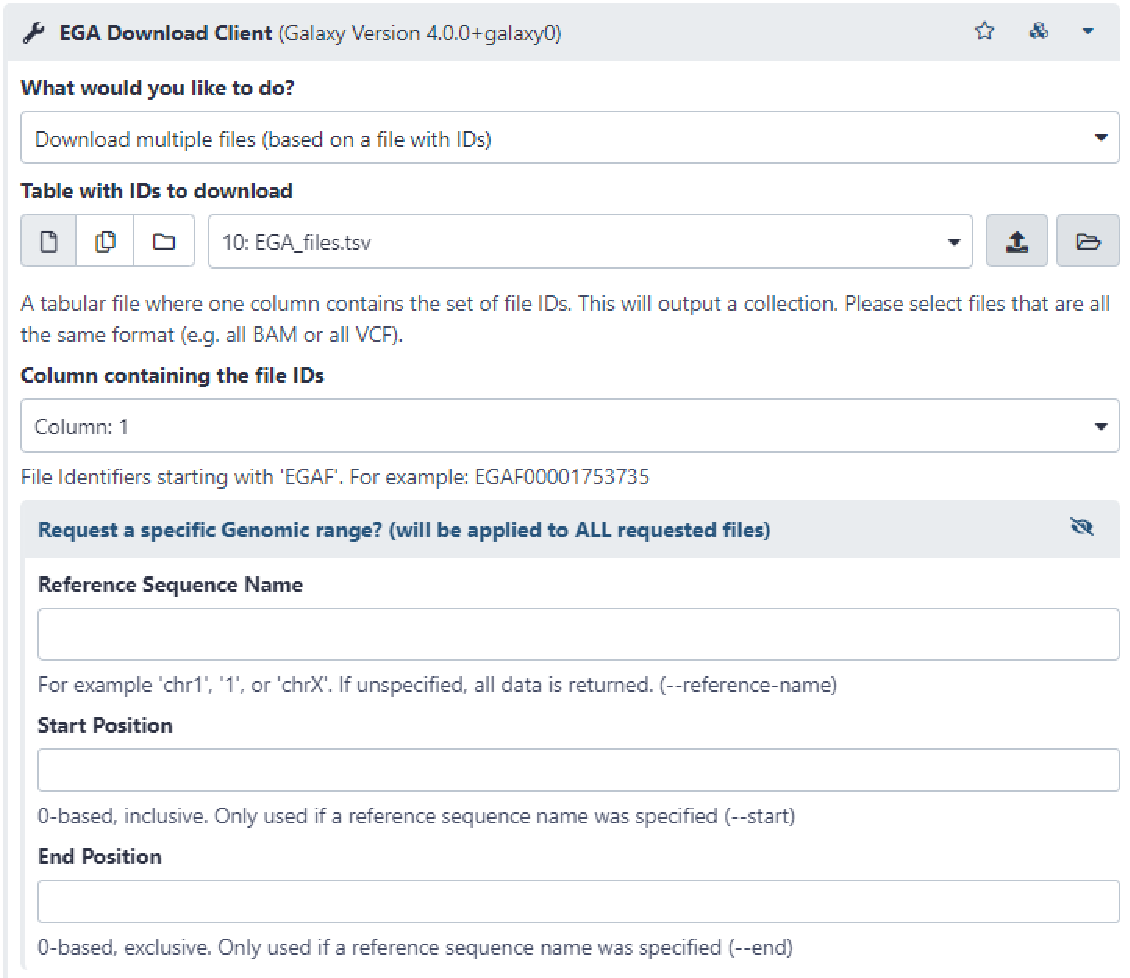
\includegraphics[width=\linewidth]{chapters/images/htsget/figure1.pdf}
    \caption{The Galaxy interface of the added feature to the PyEga3 tool to download multiple files. It takes a tabular data with EGAF IDs. In addition, a region can be provided to download a small region in BAMs or VCFs.}\label{fig:pyega}
\end{figure}

\subsubsection*{Clin.iobio}
We also implemented the gene.iobio tool within the Galaxy framework. Gene.iobio is a tool for precision genomics. The tool is able to create dynamic results, which include creating a list of genes for the disease of interest, creating an automatic report of pathogenic variants within the list of genes, allowing the custom filtering of pathogenic variants, reporting phenotypes and publications related to the gene of interest, and reviewing the variants. These are major improvements compared to the existing trio analysis tool within Galaxy, GEMINI \cite{gemini}, which was only able to produce static plots or large lists of filtered variants.

\subsubsection*{Workflow \& Tutorial}
In this study we illustrate an end-to-end workflow for trio analysis for FAIR data. This workflow retrieves and analyses files from large datasets in the EGA and can easily be adapted to any other EGA dataset. We illustrate this by analysing data from the EGAD00001008392 \cite{egad} dataset. This dataset contains 6 trio families with different inheritance patterns of digitally spiked-in variants, where each family is subject to a different disease. Next, we demonstrate the usefulness of gene.iobio by analysing the family trios and comparing the existing trio analysis tool in Galaxy, GEMINI, to the gene.iobio tool. Finally, a comprehensive tutorial is made available at the Galaxy Training materials \cite{GTN_web} under the topic `Variant Analysis` titled `Trio Analysis using Synthetic Datasets from RD-Connect GPAP)` \cite{tutorial} to teach users how to access data from the EGA and to recreate and run the workflow from scratch. In addition, the workflow is available at WorkflowHub \cite{workflowhub-wf}.

\subsubsection*{Use Case: Breast Cancer}
Here we report on the output produced by gene.iobio to demonstrate it's added value to the Galaxy platform. To produce these results we used case 5 from the EGA dataset. This case describes a family trio where the mother and daughter are affected by breast cancer. The case describes an autosomal dominant inheritance pattern, which causes a missense single nucleotide polymorphism (SNP) at chromosome 17 position 41,215,920 changing a guanine into a thymine. \cite{egad}

The BAMs and VCFs of the family trio are first downloaded using the PyEGA3 tool in Galaxy. The tool was able to securely download the trios' VCFs and slices of the large BAMs by selecting chromosome 17.
After downloading the data from the EGA the workflow pre-processes the data and produces multiple outputs using gene.iobio.

% Generated list of genes
Firstly, a disease/phenotype of interest can be provided to produce a list of genes of interest. To generate this list of genes the gene.iobio makes use of the Phenolyzer software \cite{phenolyzer}. In this case the disease is breast cancer. The automatic selection of important genes related to the disease speeds up the process of finding causative variants. Alternatively, genes can be added manually.

% Pathogenic Variants
Next, gene.iobio searches, by default, for causative variants in the top 20 of provided list of genes by filtering all the variants in the VCFs using pre-selected, but customizable, parameters. Figure \ref{fig:variant} shows that a spiked-in causative variant was found with sufficient depth and allele counts. In addition, gene.iobio shows the quality of the variant, a pathogenicity score, the population frequency, a visualization of the inhertiance patterns, and statistics on the conservation of the variant. This information helps the user to determine the legitimacy of the variant.

\begin{figure*}[t!] %% preferably at bottom or top of column
    \centering
    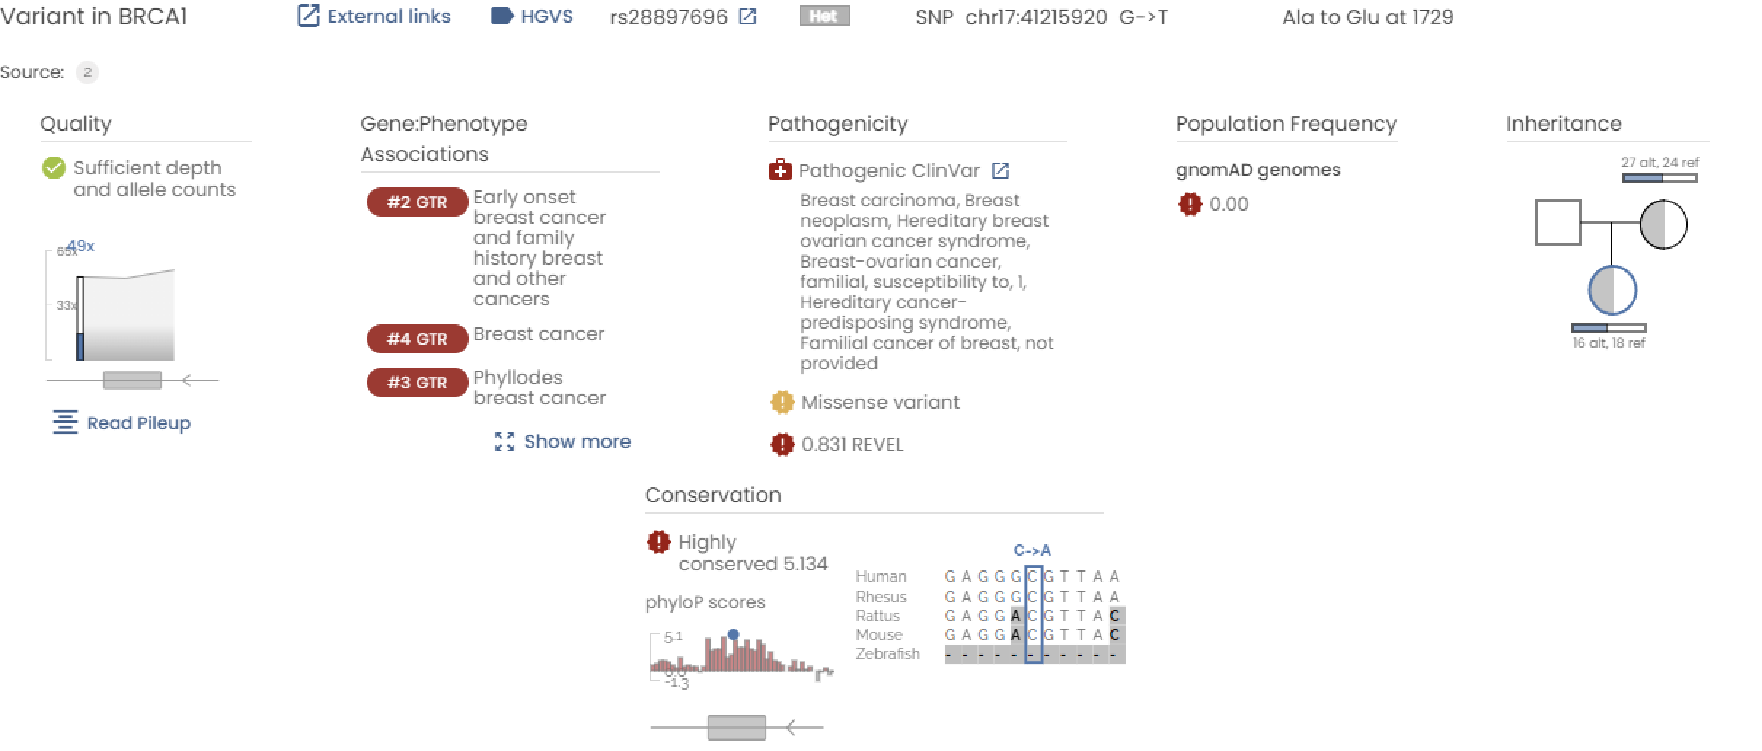
\includegraphics[width=\linewidth]{chapters/images/htsget/figure3.pdf}
    \caption{Overview of gene.iobio results for the spiked-in variant. The figure shows statistics on quality of the variant, phenotype associations, pathogenicity, population frequency, inheritance, and conservation.}\label{fig:variant}
\end{figure*}

Overall, gene.iobio provides an interactive and visual overview of causative variant identification. This is a significant improvement compared to the previous causative variant identification tool GEMINI. Especially with regards to identifying the quality of the causative variant as illustrated by figure \ref{fig:variant}.

\subsubsection*{Trio Analysis Comparison}
% Table comparing if the variant was found back
In addition, we further validated the gene.iobio tool by identifying the causative variants in all the families available. A comparison of the results reported by gene.iobio and GEMINI is shown in table \ref{tab:comparison}. It shows the number of variants reported by GEMINI and gene.iobio using the default parameters. The table shows that GEMINI does not report any variants for some cases. When GEMINI does report variants it reports the correct variants. However, it also reports many false positive, since each family has only one or two spiked-in causative variants. In contrast, gene.iobio does report causative variants for each family and only the correct ones. This shows that gene.iobio is not only interpretable but also accurate.

\begin{table}[bt!]
    \caption{Overview of existing Galaxy trio analysis tools and the number of variants they report.}\label{tab:comparison}
    \begin{tabular}{c c c}
        \toprule
        Family & GEMINI & gene.iobio \\
        \midrule
        Case1 & 0 & 1 \\ % 209  46
        Case2 & 77 & 1 \\ % 23  12
        Case3 & 0 & 2 \\ % 6    1
        Case4 & 26 & 1 \\ % 401  233
        Case5 & 142 & 1 \\ % 8  3
        Case6 & 0 & 1 \\ % 146   89
        \bottomrule
    \end{tabular}
    % \begin{tablenotes}
        % \item \textsuperscript{*} For these cases the gene of interest was not present in the gene list based on phenotypes in gene.iobio.
        % \item \textsuperscript{+} For these cases more possible causative variants were reported than expected.
    % \end{tablenotes}
\end{table}

\section*{Limitations \& Future Work}
\subsection*{PyEGA Passports}
In the current implementation of PyEGA3 in Galaxy we miss the support of authentication with Passports, a Global Alliance for Genomics and Health (GA4GH) standard. The GA4GH has developed a set of standards to facilitate data sharing within a federated context.
To access federated resources and controlled access data, the identity of the user accessing the data must be determined, along with any data access permissions the user has for particular datasets. Two GA4GH standards facilitate this, the AAI standard, and the Passport standard.
The AAI specification profiles OpenID Connect (OIDC) protocol to provide a mechanism for interoperability of identities between different institutions, supporting federated data access while ensuring the security of the data by defining the way identities and access permissions are exchanged between resources. 
The Passport standard defines how the permissions are represented, in the form of visas. There are 5 types of visa, ControlledAccessGrants which list the access permissions for the user to controlled access datasets, LinkedIdentities which allow a user to link different identities to facilitate single sign on, as well as AffiliationAndRole, AcceptedTermsAndPolicies, and ResearcherStatus.
Passports support tiered access - open, registered, and controlled. Typically, the data available to the user will increase and the user moves from open to controlled access. Any user can access resources on the open access tier, while ResearcherSatus indicates the user can access resources at the registered access tier, and ControlledAccessGrants indicate which controlled access resources the user can access. 
The Life Science AAI supports GA4GH AAI and Passport standards. A user can link their Life Science identity with one or more institutional or social media identities, and utilise these identities to access resources, such as Galaxy instances or datasets from the EGA. For example, a user can use their linked institutional identity via the Life Science AAI to access data from EGA via the EGA Permissions API and Data API. In the future, we aim to implement the Passport protocol into Galaxy to access data compliant with the GA4GH standards \cite{GA4GH}.

% Limitations Galaxy. Secure data storage
\subsection*{Data Management}
In addition to secure data retrieval, Galaxy is working on improving secure data management. Currently, data is stored unencrypted on the user's Galaxy account. But, with PyEGA implemented in Galaxy, confidential data from the EGA could be left unprotected when uploaded to a public Galaxy server. This would violate the EGA Data Access Agreement (DAA) which requires the user's institution to preserve the confidentiality of the data. %\cite{daa}

Our approach for processing confidential human genetic data would currently only be in compliance with EGA guidelines and the General Data Protection Regulation (GDPR) \cite{GDPR} when data is stored on a private Galaxy managed by the user's institution. However, data privacy at rest does exist within the community, currently S3 buckets \cite{S3_buckets} can be leveraged by Galaxy, which offer the ability to encrypt data at rest. In the future Galaxy's Crypt4GH \cite{galaxy_crypt4gh} integration project will provide a more deeply integrated alternative. This ongoing project aims to implement Crypt4GH \cite{crypt4gh}, a standardized encryption tool for genetic data, to encrypt data at rest in Galaxy automatically. Currently, this project does not consider memory encryption as every individual tool that works with the data must implement support for trusted compute. Alternatively, directories could be encrypted using a user key this would ensure the cached data is also encrypted.

\subsection*{Data Sharing}
Once EGA data has been uploaded to a Galaxy instance the data and analysis can easily be shared with other users. Currently, a user could share a history containing authenticated EGA data with another user, which does not have DAC access, which is in violation with the DAA. % ``The User Institution agrees only to transfer or disclose these Data, in whole or part, or any material derived from these Data, to the Authorised Personnel. Should the User Institution wish to share these Data with an External Collaborator, the External Collaborator must complete a separate application for access to these Data'' \cite{daa}.
Currently, Galaxy implements the ability to control privacy of individual datasets within a history, permitting the user to share the analysis results, without sharing the private source data. However, this remains a manual process. Therefore, we propose that in the future the permission to share DAC access datasets to another Galaxy user are validated automatically. We suggest that this validation should be dataset specific e.g., statistics, figures, and workflows derived from the history should be shareable as long as it is in compliance with the DAA.

\subsection*{Linking Major Repositories}
In addition to the EGA other major data repositories exist which have not been linked to Galaxy yet, such as The Cancer Genome Atlas Program (TCGA) \cite{TCGA}. The TCGA has its own data retrieval tool, the GDC Data Transfer Tool \cite{GDC}, for which separate credentials within a user's Galaxy account have to be implemented. It would be more efficient for these repositories to support passports. This would greatly simplify the adoption of other major repositories in Galaxy in a GA4GH compliant way, ultimately increasing the adoption of FAIR data principles.

An alternative to linking the repositories to Galaxy, is to deploy a Galaxy instance where the data is stored. This would still require the Galaxy instance to download the data from the repository in the Galaxy instance, but the data will never leave the repository itself. However, this would require the data repository to have sufficient computing utilities in order to analyse the data with Galaxy. In the future this might be a better alternative to linking the repositories itself.

\section*{Conclusion}
In this study we implemented PyEGA3 in Galaxy to retrieve data from the EGA in a GA4GH compliant manner. In addition, gene.iobio was implemented to improve variant analyses in Galaxy. These tools were validated by using B1MG data from the EGA and creating a findable analysis workflow into Galaxy. This work illustrates that gene.iobio is a major improvement compared to the current trio analysis tool in Galaxy as it creates interpretable and dynamic plots. In addition, we showed that Galaxy makes it feasible and manageable for any researcher to retrieve data from the EGA securely and analyse family trio data in a FAIR manner. Not only is this work applicable to trio analysis, it is also transferable to other omics analysis, such as genome assembly, metabolomics, metagenomics, proteomics, and transcriptomics. In conclusion, this work illustrates that Galaxy is one step closer to becoming a generalised omics platform for FAIR data analysis.

\section*{Methods}
\subsection*{Implementation}
The installation and dependencies for gene.iobio are handled by Galaxy (RRID:SCR\_006281). The version of gene.iobio reported here is v4.7.1a.

\subsection*{Training Materials}
Our workflow simplifies the data collection from the EGA and the visualization and analysis of family trios. In addition, we created a tutorial for running the workflow on Galaxy. Also, the tutorial describes in detail how to gain access to datasets on the EGA to simplify the adoption of this workflow for other data on the EGA. The tutorial is available at the Galaxy training materials website \cite{tutorial}.

\subsection*{Pre-Processing}
% Pre-processing of VCFs
Firstly, a `chr` prefix is added to the first column of each chromosomal site in the VCFs, to match it with the built-in reference genome from Galaxy (hg19).
Secondly, the VCFs are normalized using bcftools \cite{bcftools}. The normalization process includes left aligning insertion or deletion and splitting multiallelic sites into biallelic records.
Thirdly, the VCFs in the EGA dataset are actually genomic variant calling format (GVCFs) files. A GVCF has a record for (almost) all sites even when no variant, denoted by <NON\_REF>, is recorded. In this study this information is not informative and slows down analysis. Therefore, the records with a <NON\_REF> site are filtered out.
Fourthly, the VCFs are merged into a single VCF based on their trio pairing using bcftools. This creates a VCF where each record also has a presence/absence column for each family pair.
Finally, the variants in the merged VCF are filtered and annotated using the SnpEff tool \cite{SnpEff} as required by GEMINI. 

\subsection*{clin.iobio}
Gene.iobio is run with the GRCh37 reference genome. The gene list is created using the phenotypes described in Additional file 1. The default search filters are used to detect the causative variant.

\subsection*{GEMINI}
For each case GEMINI (RRID:SCR\_014819) is prompted to remove low impact severity variants and to search for causative variants that match the inheritance pattern in Additional file 1. 

\section*{Availability of source code and requirements}

\subsection*{Galaxy Resources}
\begin{itemize}
    \item Galaxy Home Page: \url{https://galaxyproject.org/}
    \item Galaxy Tutorials: \url{https://training.galaxyproject.org}
    \item How to install Galaxy: \url{https://getgalaxy.org}
    \item How to install tools: \url{https://galaxyproject.org/admin/tools/add-tool-from-toolshed-tutorial/}
\item Full administrative resources: \url{https://docs.galaxyproject.org/}
    \item Galaxy Help Forum: \url{https://help.galaxyproject.org/}
    \item Connect with the Galaxy Community on Gitter Chat: \url{https://gitter.im/galaxyproject/Lobby/}
\end{itemize}

\subsection*{ToolShed}
\begin{itemize}
    \item Project name: ToolShed repositories maintained by the Intergalactic Utilities Commission 
    \item GitHub repository: \url{https://github.com/galaxyproject/tools-iuc} 
    \item ToolShed repository: \url{https://toolshed.g2.bx.psu.edu/}
    \item License: MIT
\end{itemize}

\subsection*{PyEGA3}
\begin{itemize}
    \item Project name: pyega3 - uses the EGA REST API to download authorized datasets and files
    \item GitHub repository: \url{https://github.com/galaxyproject/tools-iuc/tree/master/tools/pyega3}
    \item ToolShed repository: \url{https://toolshed.g2.bx.psu.edu/view/iuc/ega_download_client}
    \item Training Manual: \url{https://training.galaxyproject.org/training-material/topics/variant-analysis/tutorials/trio-analysis/tutorial.html}
    \item Operating system(s): Unix (Platform independent with Docker, Singularity)
    \item Other requirements: Galaxy version 22.05 or higher
    \item License: Apache-2.0
    \item RRID: SCR\_024654
\end{itemize}

\subsection*{gene.iobio}
\begin{itemize}
    \item Project name: gene.iobio - an interactive tool for variant and trio analysis
    \item GitHub repository: \url{https://github.com/galaxyproject/tools-iuc/tree/master/tools/geneiobio}
    \item ToolShed repository: \url{https://toolshed.g2.bx.psu.edu/view/iuc/geneiobio}
    \item Training Manual: \url{https://gxy.io/GTN:T00320}
    \item Operating system(s): Unix (Platform independent with Docker, Singularity)
    \item Other requirements: Galaxy version 22.05 or higher
    \item License: MIT
\end{itemize}

\section*{Availability of supporting data and materials}
% Test case 5
The data used in this study were generated by a public human WGS experiment in the Illumina Platinum initiative \cite{Eberle}, which was made available by the HapMap project \cite{HapMap}. All data from this project is available at the EGA website \cite{EGA}. In this study only the BAMs and VCFs with the chromosomes containing the spiked-in variants were included. These files are available under `RD-Connect GPAP synthetic data spiked-in variant data` at Zenodo \cite{zenodo}. Other data further supporting this work are openly available in the GigaScience repository, GigaDB \cite{gigadb}. 

\section*{Additional Files}
Additional file 1. The report describing the family trios.

\section*{Declarations}

\subsection*{List of abbreviations}
AAI: Authentication and Authorisation; BAM: Binary alignment map; B1MG: Beyond 1 Million Genomes; DAA: Data Access Agreement; DAC: Data Access Committee; EGA: European Genome-Phenome Archive; FAIR: Findable, Accessible, Interoperable, and Reusable; GA4GH: Global Alliance for Genomics and Health; GDPR: General Data Protection Regulation; GTN: Galaxy Training Network; GVCF: Genomic variant calling format; OIDC: OpenID Connect; SNP: Single nucleotide polymorphism; TCGA: The Cancer Genome Atlas Program; VCF: Variant call format.

\subsection*{Competing Interests}
The authors declare that they have no competing interests.

\subsection*{Funding}
This work has received funding from the EC H2020 project CINECA (grant 825775) \cite{CINECA} as well as the Erasmus+ programme of the European Union (Gallantries Project, grant 2020-1-NL01-KA203-064717, doi:10.13039/100001501). The data used in this project was created with the support of the RD-Connect GPAP \cite{RD_connect_GPAP}, EC H2020 project EJP-RD (grant 825575) \cite{EJP-RD}, EC H2020 project B1MG (grant 951724) \cite{B1MG_grant}, and Generalitat de Catalunya project VEIS (grant 001-P-001647) \cite{VEIS}.

\subsection*{Author's Contributions}
J.O., S.H., H.R., and D.S. contributed to writing the manuscript. J.O., S.H., H.R. contributed to writing the Galaxy workflow tutorial. S.H., H.R., and D.D. contributed to implementing the PyEGA3 and gene.iobio tool in Galaxy. A.P.S. supervised the project. All authors approved the manuscript.

\section*{Acknowledgements}
We would like to thank the Galaxy community and in particular Wolfgang Maier, for reviewing, testing, and validating the workflow tutorial, and PyEGA3.

\footnotesize
\bibliographystyle{ieeetr}
\bibliography{references}
\normalsize
